\chapter{Results}

We present the results of our performance evaluation. To assess the efficiency and improvements brought by the parallel CUDA implementation, we tested the algorithm on three different machines, each with distinct hardware specifications. 

For each machine, we conducted six tests with varying configurations, including different image sizes, numbers of clusters, and thread configurations. This allowed us to analyze how the algorithm scales with different hardware and computational loads.

The three tested machines are as follows:

\begin{itemize}
    \item \textbf{Machine 1:} Equipped with an \textbf{NVIDIA GeForce GTX 1660} GPU (Turing architecture, 1536 CUDA cores, 6GB GDDR5 VRAM) and an \textbf{Intel Core i5-9600K} CPU (6 cores, 6 threads, 2.2GHz). This represents a mid-range consumer-grade system.
    
    \item \textbf{Machine 2:} Featuring an \textbf{NVIDIA GeForce RTX 4060} GPU (Ada Lovelace architecture, 3072 CUDA cores, 8GB GDDR6 VRAM) and an \textbf{AMD Ryzen 5 3600} CPU (6 cores, 12 threads, 2.2GHz). This machine is the most powerful among the tested ones, providing insights into high-performance configurations.

    \item \textbf{Machine 3:} A workstation-class system with an \textbf{NVIDIA Quadro K5000} GPU (Kepler architecture, 1536 CUDA cores, 4GB GDDR5 VRAM) and an \textbf{Intel Core i7} CPU (4 cores, 2.8GHz). This represents an older generation of hardware, providing a benchmark for performance on legacy systems.
\end{itemize}

The following subsections present and analyze the execution times and speedups achieved under different configurations.

\section{How the results are collected}
Each session folder has a README.md file that contains the main results of the session such as execution time, speedup, output image yielded by the program, and so on.

An advanced insights are contained in the binary files named report.ncu-rep, theese files provid detailed information about the execution of the CUDA kernels, in this way we were able to analyze common issues about CUDA kernels, such as bottleneck problem.

The report.ncu-rep files were generated using NVIDIA Nsight Compute, so to read it you have to install this tool, then you have to launch the follow command on your terminal:

\begin{lstlisting}[basicstyle=\ttfamily\footnotesize\color{white}, backgroundcolor=\color{black}, keywordstyle=\color{white}, stringstyle=\color{white}, identifierstyle=\color{white}]
    ncu-ui "report.ncu-rep"
\end{lstlisting}





For the GPUs that has a compute capability lower than 7.0 we weren't able to use Nsight Compute, for this reason we have used nvprof tool to collect insights on theese generation of GPUs; nvprof profiling are stored in the files called output.nvprof.
The results are visualizable only using NVIDIA Visual Profiler. Anyway a profiler.output.txt file has been generated for summary insights.



\section{Test 1}
\begin{figure}[H]
    \centering
    \begin{minipage}[b]{0.45\textwidth}
        \centering
        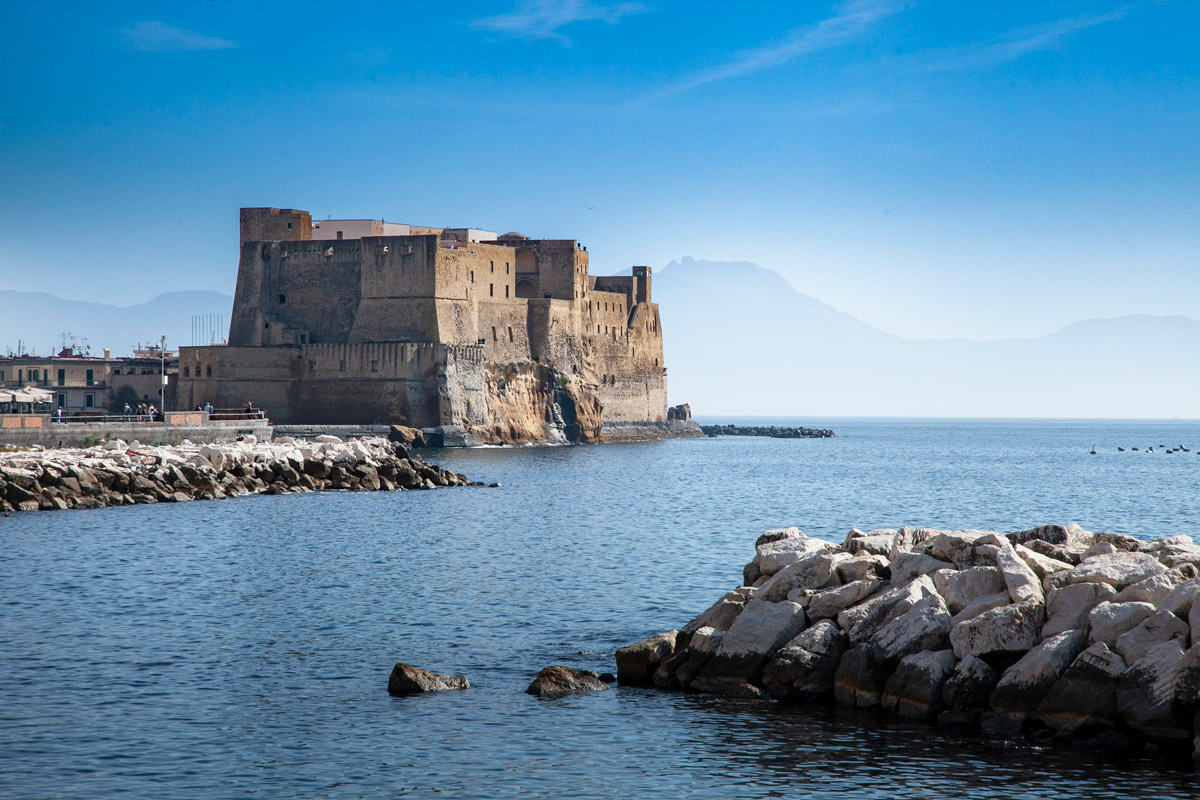
\includegraphics[width=\textwidth]{images/input_image_t1.jpg}
        \caption{(a) Input image.}
        \label{fig:test_1_input}
    \end{minipage}
    \hfill
    \begin{minipage}[b]{0.45\textwidth}
        \centering
        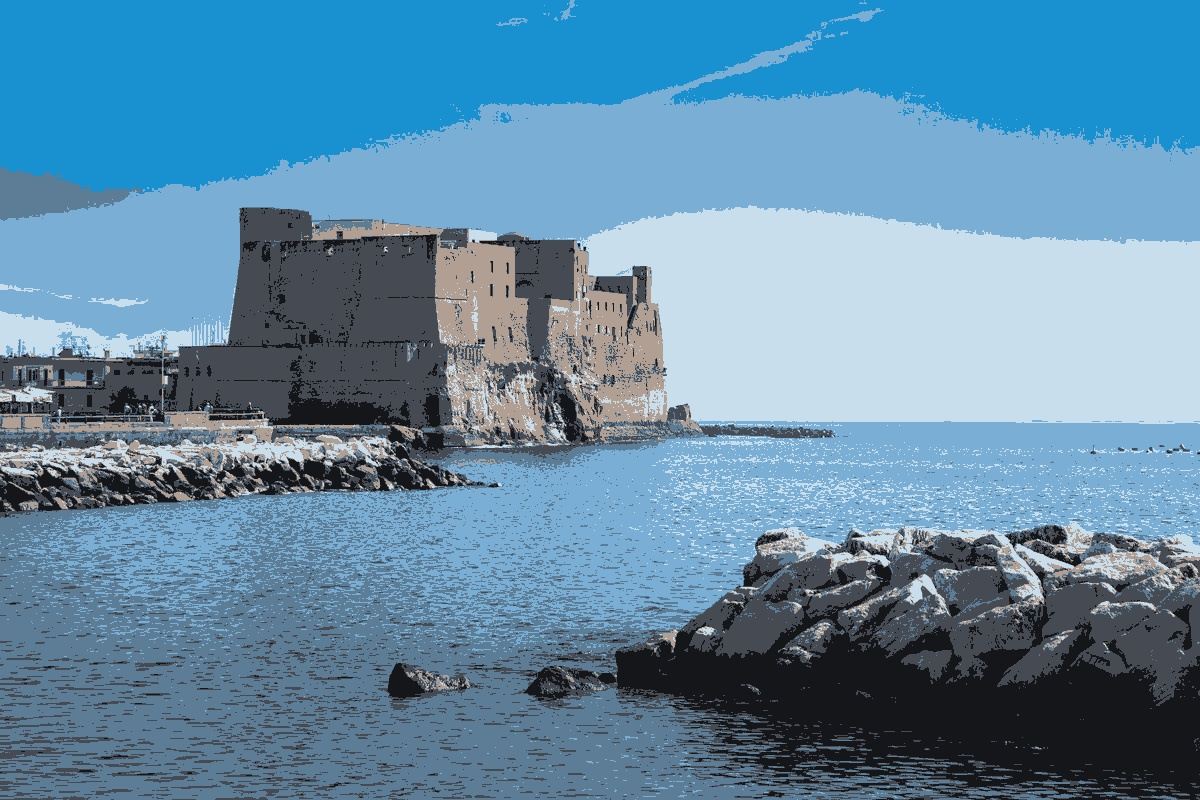
\includegraphics[width=\textwidth]{images/output_image_t1.jpg}
        \caption{(b) Output image.}
        \label{fig:test_1_output}
    \end{minipage}
    \end{figure}
    
\begin{table}[H]
    \centering
    \begin{tabular}{|l|l|}
    \hline
    \textbf{Input Info} & \textbf{Value} \\ \hline
    Session ID          & 0              \\ \hline
    Image width         & 1200px         \\ \hline
    Image height        & 800px          \\ \hline
    Image channels      & RGB (3 channels) \\ \hline
    \#Clusters          & 7              \\ \hline
    \#Iterations        & 50             \\ \hline
    \#Threads           & 256            \\ \hline
    Random seed         & 200            \\ \hline
    \end{tabular}
    \caption{Session information}
    \label{table:session_information_test1}
    \end{table}
    
\subsection{GeForce 1660}

    \begin{table}[H]
        \centering
        \begin{tabular}{|l|l|}
        \hline
        \textbf{Metric}                     & \textbf{Value}                \\ \hline
        Execution time (Parallel version)   & ~569ms (0.59s)                \\ \hline
        Execution time (Sequential version) & ~5034ms (5s)                  \\ \hline
        Delta time                          & +4438ms (+4.4s)               \\ \hline
        Speedup                             & 8.84                          \\ \hline
        \end{tabular}
        \caption{Performance Metrics on \textbf{Machine 1}}
        \label{table:performance_metrics_test1_machine1}
        \end{table}
        

\subsection{Geforce 4060}
\begin{table}[H]
    \centering
    \begin{tabular}{|l|l|}
    \hline
    \textbf{Metric}                         & \textbf{Value}                       \\ \hline
    Execution time (Parallel version)       & ~450ms (0.45s)                        \\ \hline
    Execution time (Sequential version)     & ~4000ms (4s)                          \\ \hline
    Delta time                               & +3550ms (+3.5s)                       \\ \hline
    Speedup                                  & 8.8                                   \\ \hline
    \end{tabular}
    \caption{Performance Metrics on \textbf{Machine 2}}
    \label{tab:performance_metrics_test1_machine2}
    \end{table}
    
\subsection{Quadro K5000}
\begin{table}[H]
    \centering
    \begin{tabular}{|l|l|}
    \hline
    \textbf{Metric}                         & \textbf{Value}                       \\ \hline
    Execution time (Parallel version)       & ~1451ms (1.45s)                       \\ \hline
    Execution time (Sequential version)     & ~11630ms (11.63s)                     \\ \hline
    Delta time                               & +10179ms (+10.17s)                    \\ \hline
    Speedup                                  & 8                                     \\ \hline
    \end{tabular}
    \caption{Performance Metrics on \textbf{Machine 3}}
    \label{tab:performance_metrics_test1_machine3}
    \end{table}
    
\subsection{Conclusion}
In conclusion, the results from the three different machines show varied performance metrics with respect to execution time, speedup, and efficiency. As expected, the parallel version of the task consistently outperforms the sequential version in all cases, with the speedup ranging from 8x to 9x across the tested machines. 

The GeForce 1660 machine performed well with a speedup of 8.84, while the Geforce 4060 machine showed a slightly lower speedup of 8.8. Interestingly, the Quadro K5000 machine, while having a significant sequential execution time, achieved a speedup of 8. This shows the importance of parallelization in reducing the processing time on different hardware configurations. Further tests with different image sizes or more threads could provide even more insights into how well these machines scale with different workloads.

The parallel implementation not only demonstrated a clear advantage in terms of speedup but also allowed the machines to efficiently handle larger input sizes, further highlighting the importance of parallel computation in modern hardware environments.

\section{Test 2}
\begin{figure}[H]
    \centering
    \begin{minipage}[b]{0.45\textwidth}
        \centering
        
\includegraphics[width=\textwidth]{images/input_image_t2.jpg}
        \caption{(a) Input image.}
        \label{fig:test_2_input}
    \end{minipage}
    \hfill
    \begin{minipage}[b]{0.45\textwidth}
        \centering
        \includegraphics[width=\textwidth]{images/output_image_t2.jpg}
        \caption{(b) Output image.}
        \label{fig:test_2_output}
    \end{minipage}
    \end{figure}

    \begin{table}[H]
        \centering
        \begin{tabular}{|l|l|}
        \hline
        \textbf{Input Info}                    & \textbf{Value}                       \\ \hline
        Session ID                             & 1                                     \\ \hline
        Image width                            & 7680px                                \\ \hline
        Image height                           & 4320px                                \\ \hline
        Image channels                         & RGB (3 channels)                      \\ \hline
        \#Clusters                             & 7                                     \\ \hline
        \#Iterations                           & 50                                    \\ \hline
        \#Threads                              & 256                                   \\ \hline
        Random seed                            & 200                                   \\ \hline
        \end{tabular}
        \caption{Session information}
        \label{tab:session_information_test2}
        \end{table}
        

        \subsection{GeForce 1660}

        \begin{table}[H]
            \centering
            \begin{tabular}{|l|l|}
            \hline
            \textbf{Metric}                         & \textbf{Value}                       \\ \hline
            Execution time (Parallel version)       & ~19885ms (19.88s)                     \\ \hline
            Execution time (Sequential version)     & ~163264ms (2.7 minutes)               \\ \hline
            Delta time                               & +143379ms (+2.38 minutes)             \\ \hline
            Speedup                                  & 8.21                                   \\ \hline
            \end{tabular}
            \caption{Performance Metrics on \textbf{Machine 1}}
            \label{table:performance_metrics_test2_machine1}
        \end{table}
        
        
        \subsection{Geforce 4060}
        
        \begin{table}[H]
            \centering
            \begin{tabular}{|l|l|}
            \hline
            \textbf{Metric}                         & \textbf{Value}                       \\ \hline
            Execution time (Parallel version)       & ~19000ms (19s)                        \\ \hline
            Execution time (Sequential version)     & ~150000ms (2.5 minutes)               \\ \hline
            Delta time                               & +148000ms (+1.40 minutes)            \\ \hline
            Speedup                                  & 78.94                                  \\ \hline
            \end{tabular}
            \caption{Performance Metrics on \textbf{Machine 2}}
            \label{table:performance_metrics_test2_machine2}
        \end{table}
        
        
        \subsection{Quadro K5000}
        
        \begin{table}[H]
            \centering
            \begin{tabular}{|l|l|}
            \hline
            \textbf{Metric}                         & \textbf{Value}                       \\ \hline
            Execution time (Parallel version)       & ~50608ms (50.60s)                     \\ \hline
            Execution time (Sequential version)     & ~398440ms (6.64 minutes)              \\ \hline
            Delta time                               & +347832ms (+5.79 minutes)            \\ \hline
            Speedup                                  & 7.87                                   \\ \hline
            \end{tabular}
            \caption{Performance Metrics on \textbf{Machine 3}}
            \label{table:performance_metrics_test2_machine3}
        \end{table}

\subsection{Conclusion}
In Test 2, we observed significant improvements in performance across all three machines tested, particularly in the parallel execution versions. The GeForce 1660 achieved a speedup of 8.21, with a substantial reduction in execution time compared to the sequential version. The Geforce 4060 showed an even more impressive performance with a speedup of 78.94, demonstrating its strong ability to handle parallel tasks efficiently. Meanwhile, the Quadro K5000, while lagging behind in speedup at 7.87, still exhibited a noteworthy improvement over the sequential execution.

These results emphasize the importance of parallel processing, especially when dealing with larger image sizes and complex computations. The differences in performance between the machines highlight the varying capabilities of the hardware, with newer or more powerful GPUs (like the Geforce 4060) offering a much greater reduction in processing time compared to older models. Overall, the parallel implementation proved to be highly effective, achieving notable speedups in all cases, and further optimization could push these numbers even higher.

\section{Test 3}
\begin{figure}[H]
    \centering
    \begin{minipage}[b]{0.45\textwidth}
        \centering
        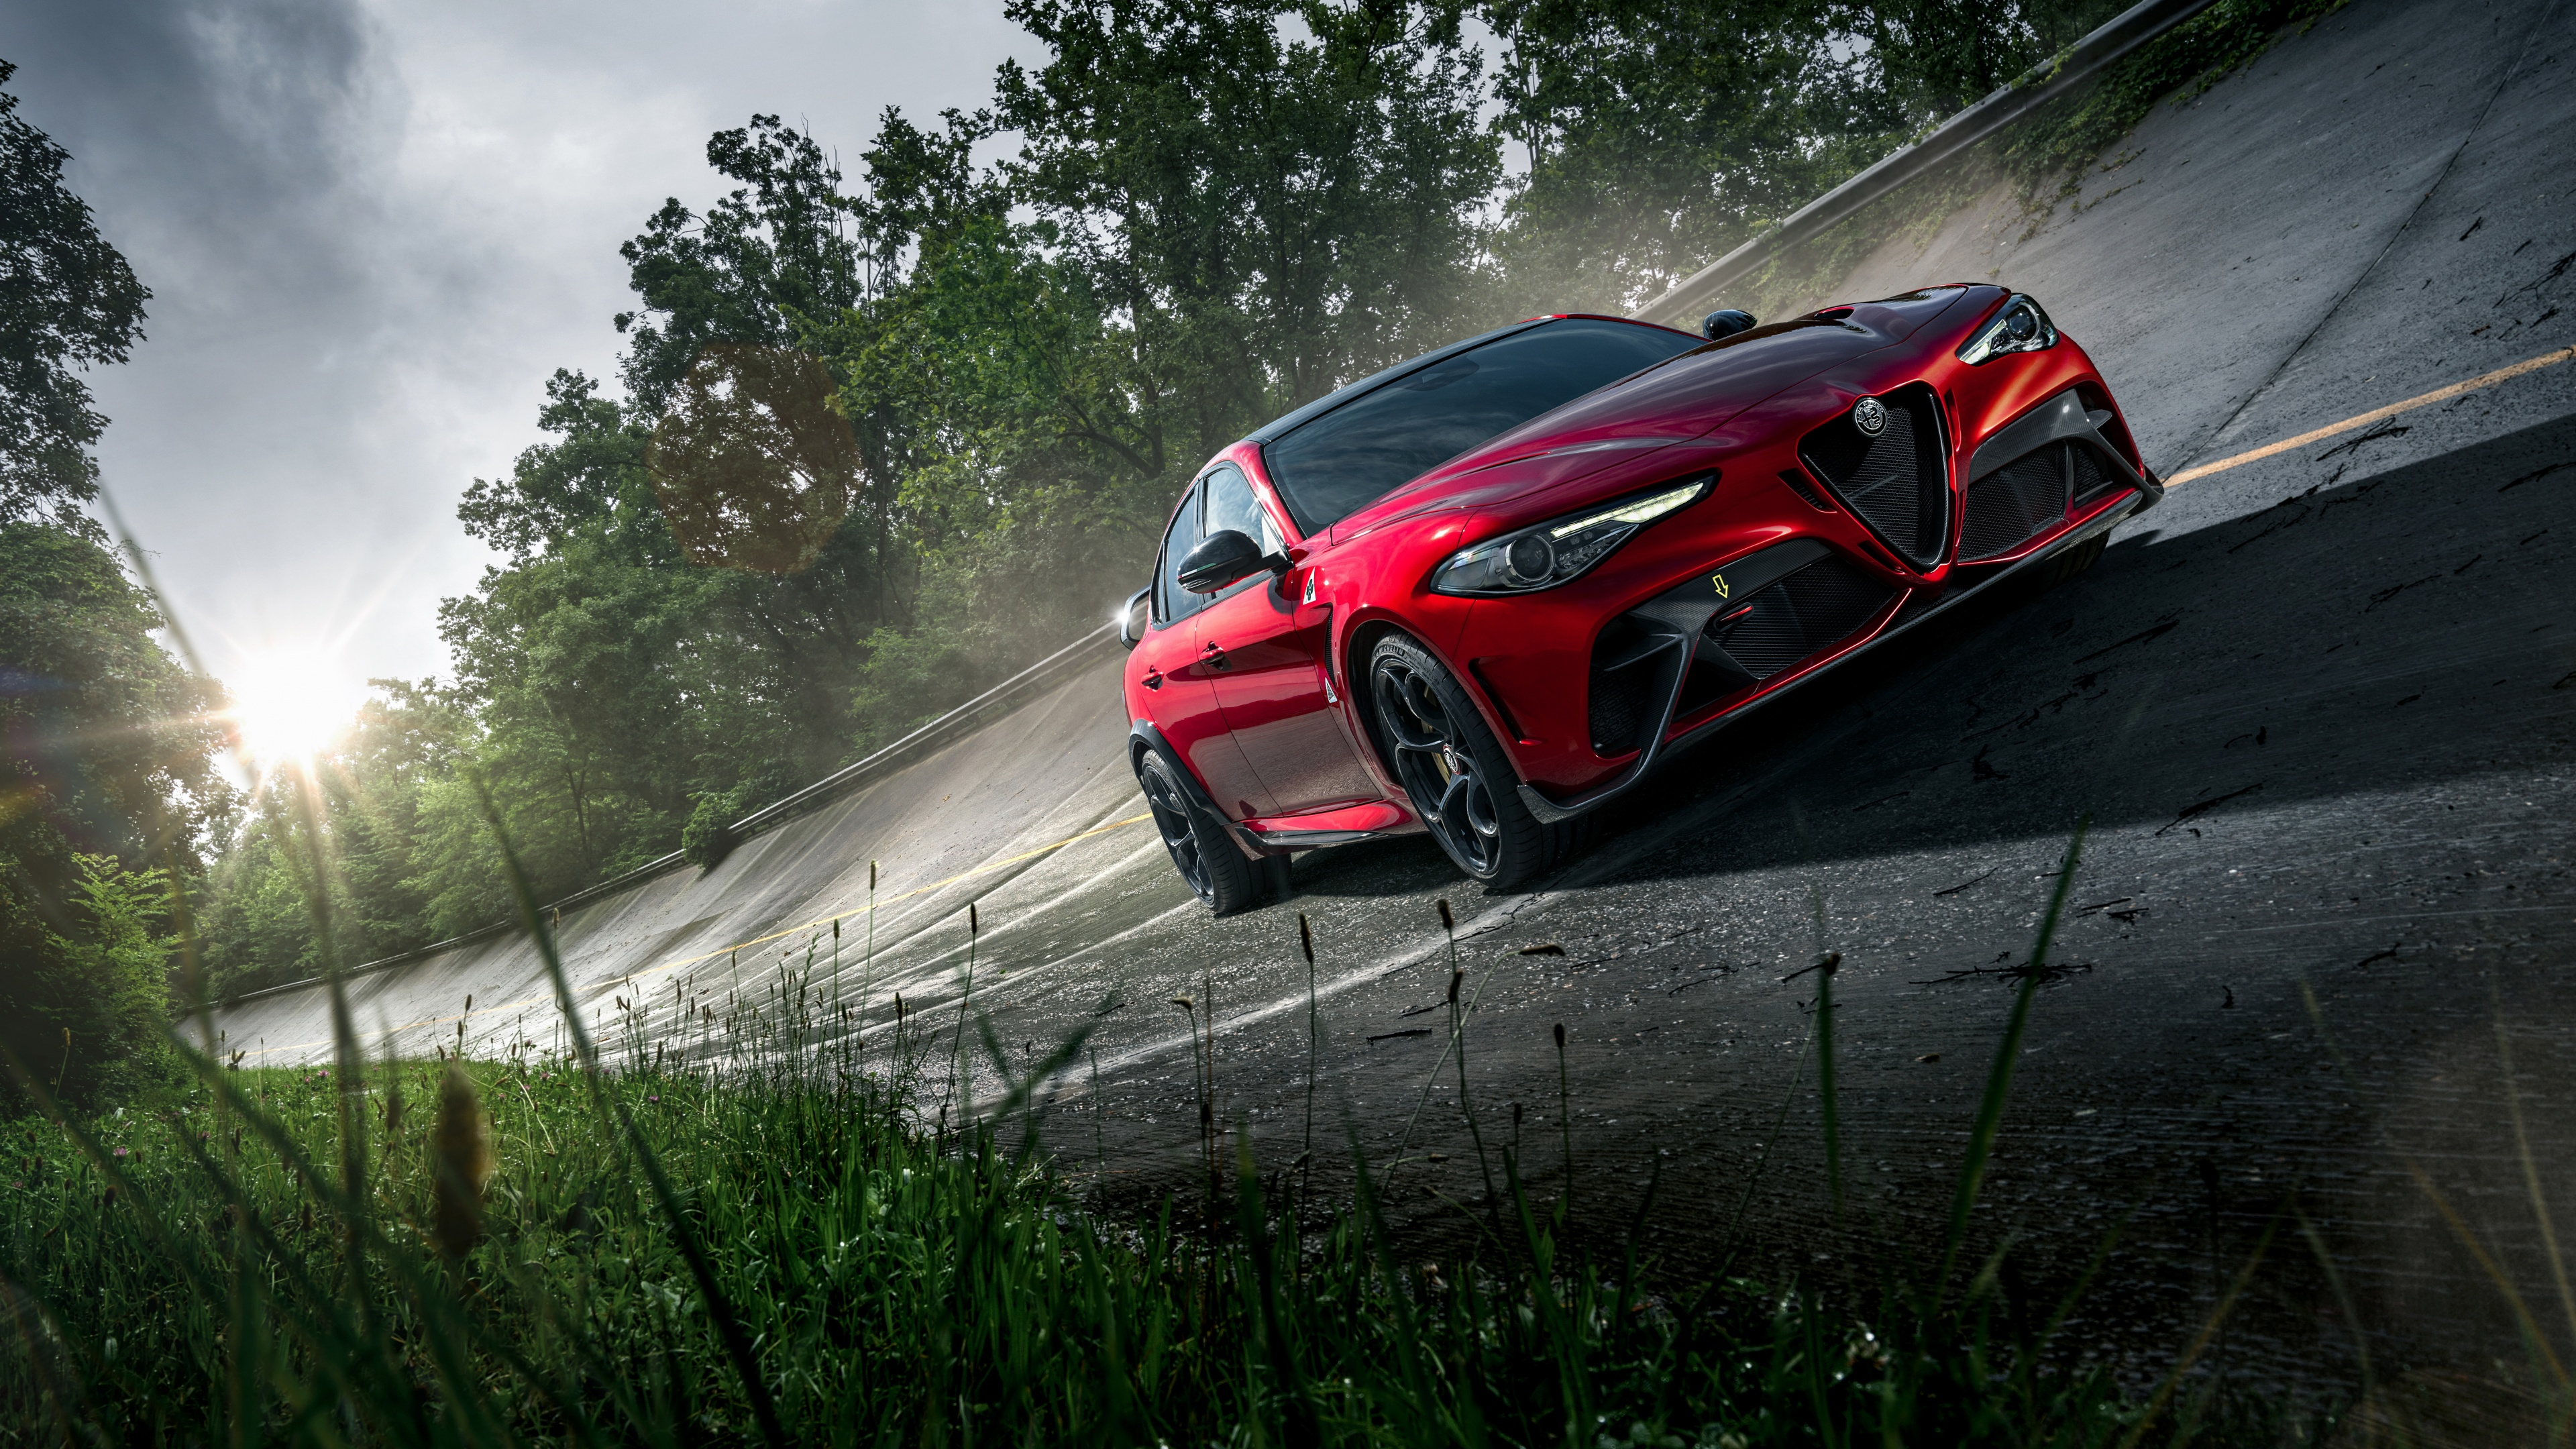
\includegraphics[width=\textwidth]{images/input_image_t3.jpg}
        \caption{(a) Input image.}
        \label{fig:test_3_input}
    \end{minipage}
    \hfill
    \begin{minipage}[b]{0.45\textwidth}
        \centering
        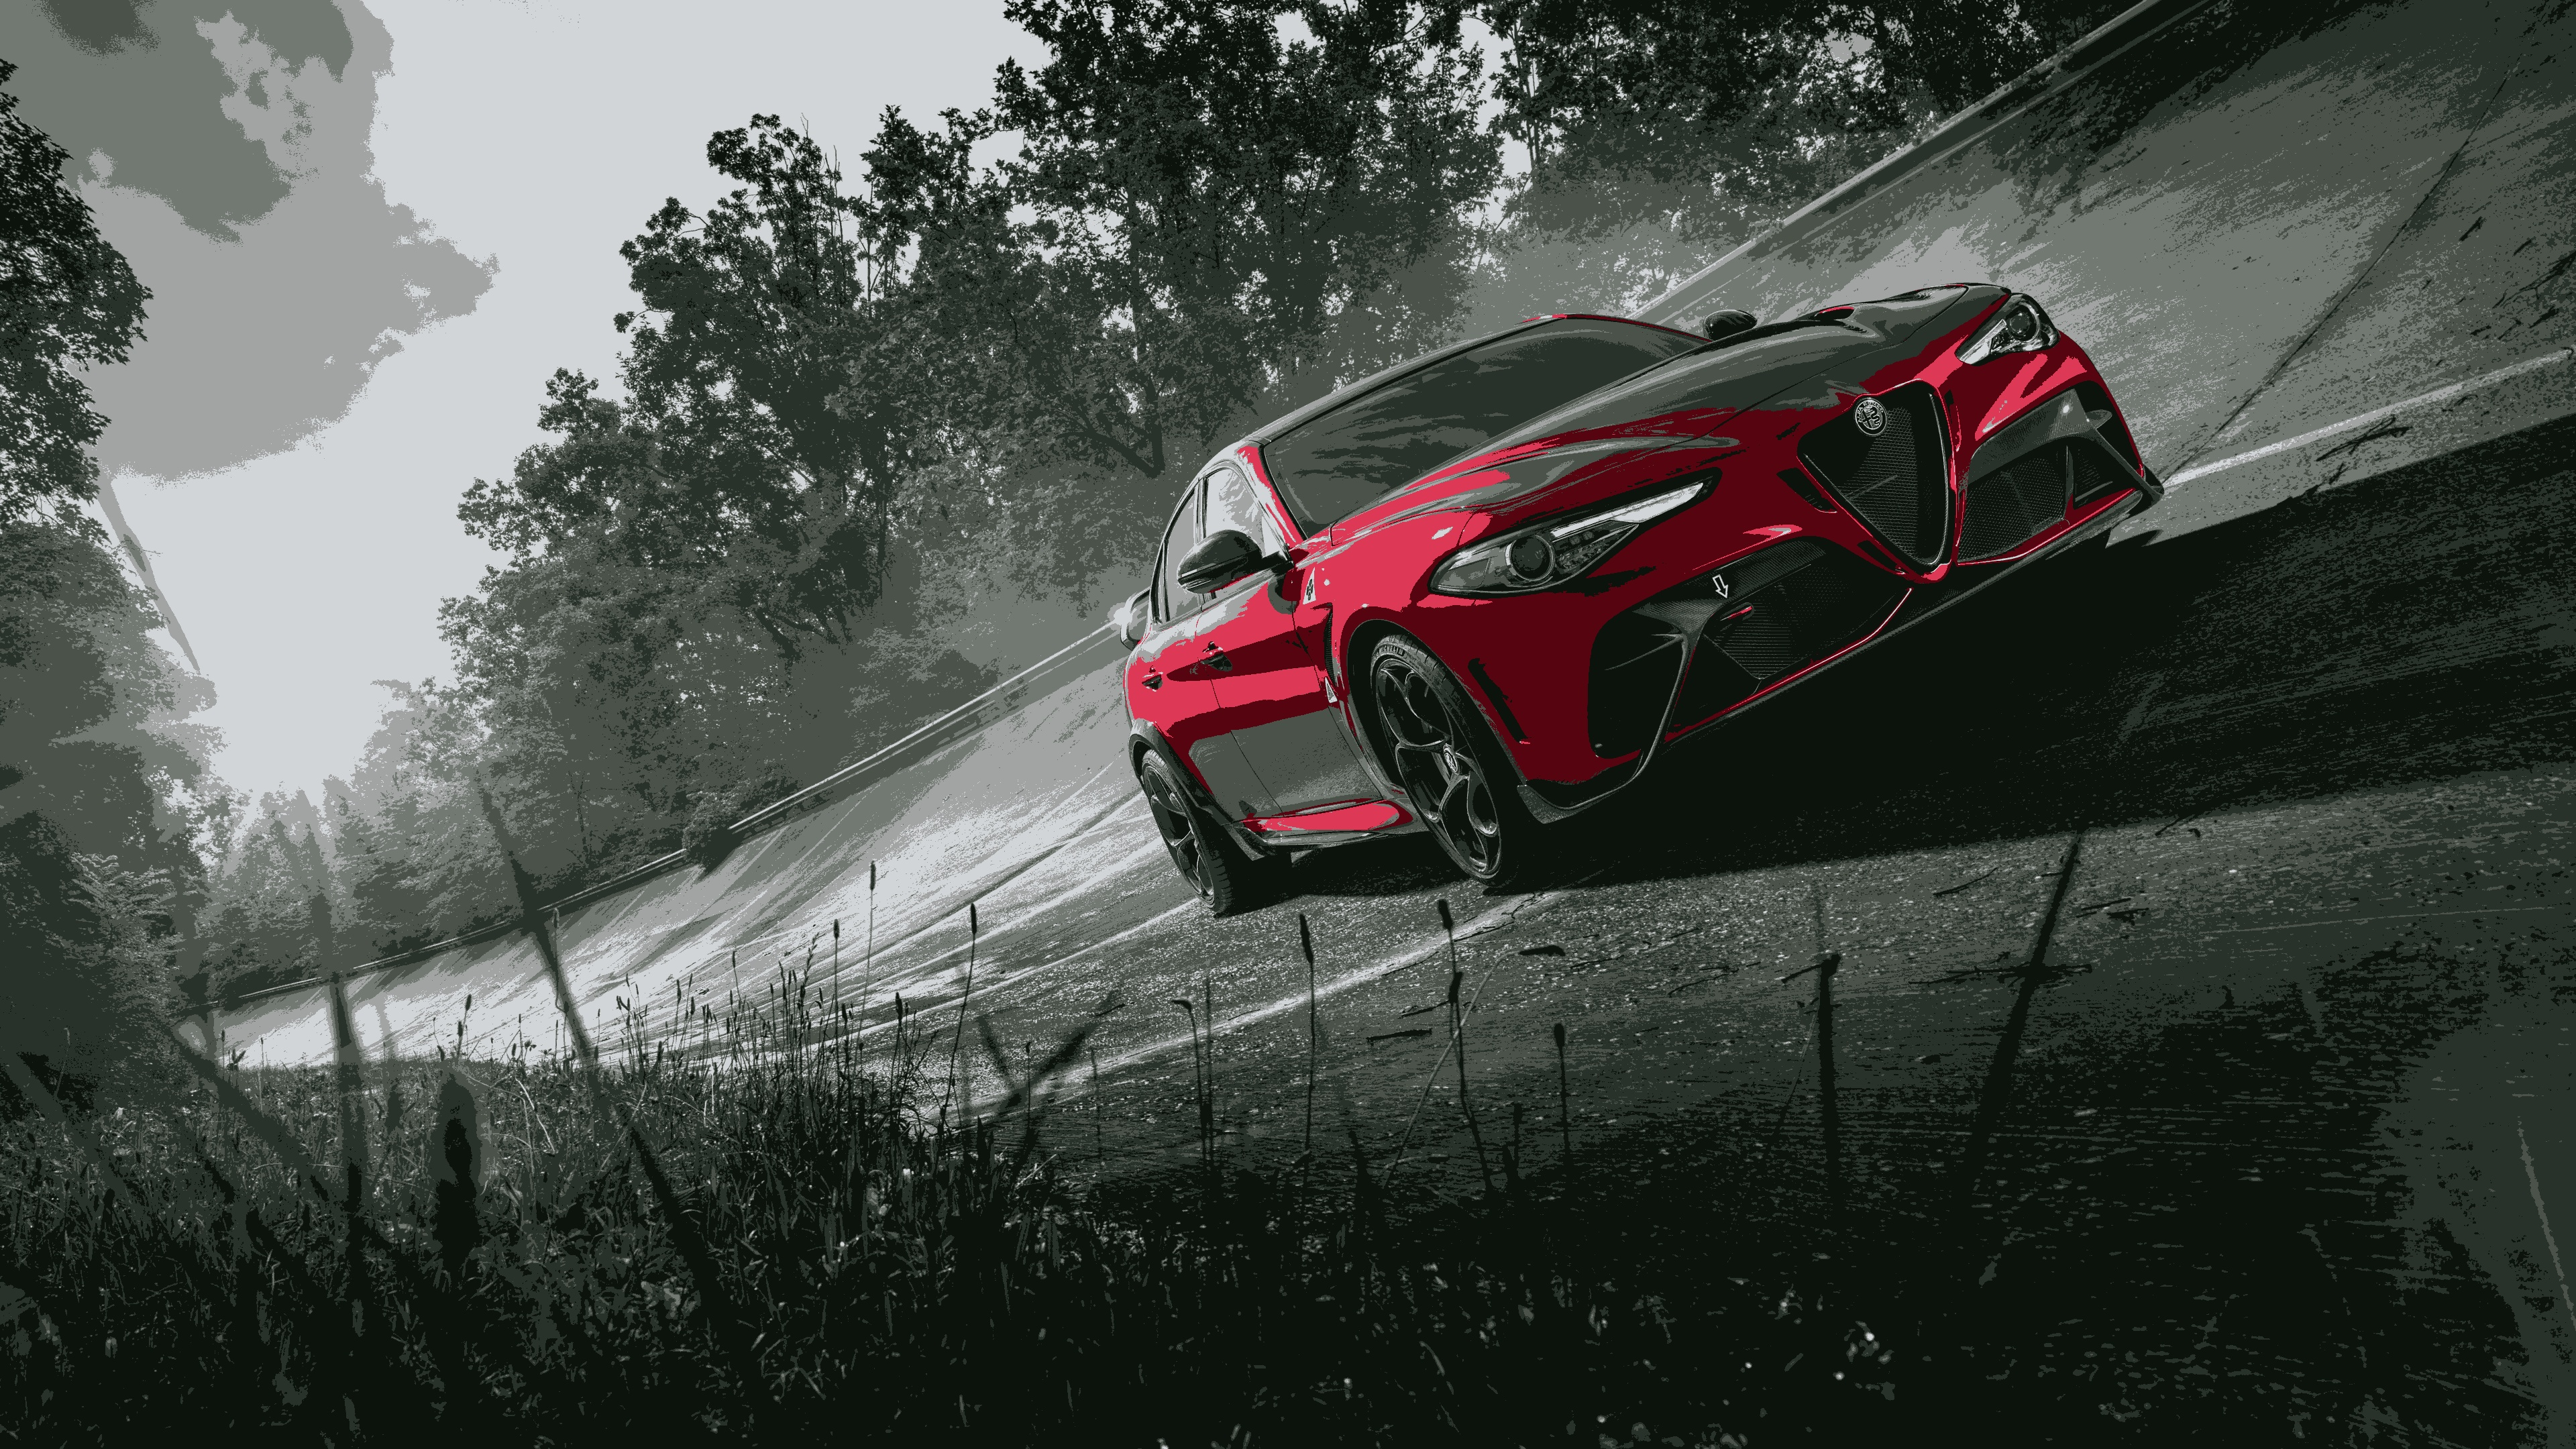
\includegraphics[width=\textwidth]{images/output_image_t3.jpg}
        \caption{(b) Output image.}
        \label{fig:test_3_output}
    \end{minipage}
    \end{figure}

    \begin{table}[H]
        \centering
        \begin{tabular}{|l|l|}
        \hline
        \textbf{Input Info}                    & \textbf{Value}                       \\ \hline
        Session ID                             & 2                                     \\ \hline
        Image width                            & 3840px                                \\ \hline
        Image height                           & 2160px                                \\ \hline
        Image channels                         & RGB (3 channels)                      \\ \hline
        \#Clusters                             & 8                                     \\ \hline
        \#Iterations                           & 50                                    \\ \hline
        \#Threads                              & 128                                   \\ \hline
        Random seed                            & 200                                   \\ \hline
        \end{tabular}
        \caption{Session information}
        \label{tab:session_information_test3}
        \end{table}
        
        \subsection{GeForce 1660}

        \begin{table}[H]
            \centering
            \begin{tabular}{|l|l|}
            \hline
            \textbf{Metric}                         & \textbf{Value}                       \\ \hline
            Execution time (Parallel version)       & ~4397ms (4.39s)                       \\ \hline
            Execution time (Sequential version)     & ~41379ms (41.37s)                     \\ \hline
            Delta time                               & +36982ms (+36.98s)                    \\ \hline
            Speedup                                  & 9.4                                    \\ \hline
            \end{tabular}
            \caption{Performance Metrics on \textbf{Machine 1}}
            \label{table:performance_metrics_test3_machine1}
        \end{table}
        
        
        \subsection{Geforce 4060}
        
        \begin{table}[H]
            \centering
            \begin{tabular}{|l|l|}
            \hline
            \textbf{Metric}                         & \textbf{Value}                       \\ \hline
            Execution time (Parallel version)       & ~4265ms (4s)                          \\ \hline
            Execution time (Sequential version)     & ~43369ms (43s)                        \\ \hline
            Delta time                               & +39000ms (+39s)                       \\ \hline
            Speedup                                  & 10.17                                  \\ \hline
            \end{tabular}
            \caption{Performance Metrics on \textbf{Machine 2}}
            \label{table:performance_metrics_test3_machine2}
        \end{table}
        
        
        \subsection{Quadro K5000}
        
        \begin{table}[H]
            \centering
            \begin{tabular}{|l|l|}
            \hline
            \textbf{Metric}                         & \textbf{Value}                       \\ \hline
            Execution time (Parallel version)       & ~12030ms (12.03s)                     \\ \hline
            Execution time (Sequential version)     & ~105250ms (1.75 minutes)             \\ \hline
            Delta time                               & +93220ms (+1.55 minutes)             \\ \hline
            Speedup                                  & 8.74                                   \\ \hline
            \end{tabular}
            \caption{Performance Metrics on \textbf{Machine 3}}
            \label{table:performance_metrics_test3_machine3}
        \end{table}

\subsection{Conclusion}
In Test 3, we observed consistent improvements in execution times across all machines when using parallel processing. The GeForce 1660 achieved a speedup of 9.4, significantly reducing the time taken compared to the sequential version. The Geforce 4060 performed even better, with a speedup of 10.17, highlighting its ability to handle parallel tasks efficiently. Meanwhile, the Quadro K5000, although showing a lower speedup of 8.74, still demonstrated a notable reduction in processing time.

These results reinforce the effectiveness of parallel computation, especially in handling larger images. While the newer GPUs (Geforce 4060) exhibit higher speedups, all tested machines benefited from the parallel version, making this approach highly valuable for performance optimization. The differences in speedup across different hardware platforms suggest that further optimization could yield even more impressive results, especially on more powerful machines.        

\section{Test 4}
\begin{figure}[H]
    \centering
    \begin{minipage}[b]{0.45\textwidth}
        \centering
        \includegraphics[width=\textwidth]{images/input_image_t4.jpg}
        \caption{(a) Input image.}
        \label{fig:test_4_input}
    \end{minipage}
    \hfill
    \begin{minipage}[b]{0.45\textwidth}
        \centering
        \includegraphics[width=\textwidth]{images/output_image_t4.jpg}
        \caption{(b) Output image.}
        \label{fig:test_4_output}
    \end{minipage}
    \end{figure}


    \begin{table}[H]
        \centering
        \begin{tabular}{|l|l|}
        \hline
        \textbf{Input Info}                    & \textbf{Value}                       \\ \hline
        Session ID                             & 3                                     \\ \hline
        Image width                            & 7680px                                \\ \hline
        Image height                           & 5120px                                \\ \hline
        Image channels                         & RGB (3 channels)                      \\ \hline
        \#Clusters                             & 5                                     \\ \hline
        \#Iterations                           & 50                                    \\ \hline
        \#Threads                              & 64                                    \\ \hline
        Random seed                            & 200                                   \\ \hline
        \end{tabular}
        \caption{Session information}
        \label{tab:session_information_test4}
        \end{table}
        

\subsection{GeForce 1660}

\begin{table}[H]
    \centering
    \begin{tabular}{|l|l|}
    \hline
    \textbf{Metric}                         & \textbf{Value}                       \\ \hline
    Execution time (Parallel version)       & ~23691ms (23.69s)                     \\ \hline
    Execution time (Sequential version)     & ~194534ms (3.24 minutes)              \\ \hline
    Delta time                               & +170843ms (+2.84 minutes)            \\ \hline
    Speedup                                  & 8.21                                   \\ \hline
    \end{tabular}
    \caption{Performance Metrics on \textbf{Machine 1}}
    \label{table:performance_metrics_test4_machine1}
\end{table}


\subsection{Geforce 4060}

\begin{table}[H]
    \centering
    \begin{tabular}{|l|l|}
    \hline
    \textbf{Metric}                         & \textbf{Value}                       \\ \hline
    Execution time (Parallel version)       & ~23428ms (23.4s)                      \\ \hline
    Execution time (Sequential version)     & ~138567ms (2.3 minutes)               \\ \hline
    Delta time                               & +115139ms (+1.9 minutes)              \\ \hline
    Speedup                                  & 5.9                                    \\ \hline
    \end{tabular}
    \caption{Performance Metrics on \textbf{Machine 2}}
    \label{table:performance_metrics_test4_machine2}
\end{table}


\subsection{Quadro K5000}

\begin{table}[H]
    \centering
    \begin{tabular}{|l|l|}
    \hline
    \textbf{Metric}                         & \textbf{Value}                       \\ \hline
    Execution time (Parallel version)       & ~59699ms (59.69s)                     \\ \hline
    Execution time (Sequential version)     & ~482330ms (8.3 minutes)              \\ \hline
    Delta time                               & +422631ms (+7 minutes)               \\ \hline
    Speedup                                  & 8                                     \\ \hline
    \end{tabular}
    \caption{Performance Metrics on \textbf{Machine 3}}
    \label{table:performance_metrics_test4_machine3}
\end{table}

\subsection{Conclusion}
In Test 4, we observed notable performance improvements with parallel processing across all machines. The GeForce 1660 achieved a speedup of 8.21, significantly reducing the execution time compared to the sequential version. The Geforce 4060 also demonstrated a solid performance with a speedup of 5.9, while the Quadro K5000 achieved a speedup of 8, still showing a substantial reduction in processing time.

Although the GeForce 1660 outperformed the Geforce 4060 in terms of speedup, it is clear that parallel processing is highly beneficial across all hardware tested. The difference in speedups suggests that more powerful GPUs, like the Geforce 4060, may require further optimization to fully capitalize on their potential for parallel computation. Overall, these results reinforce the importance of parallelization in reducing processing times for large-scale image tasks, offering considerable advantages over sequential execution.


\section{Test 5}
\begin{figure}[H]
    \centering
    \begin{minipage}[b]{0.45\textwidth}
        \centering
        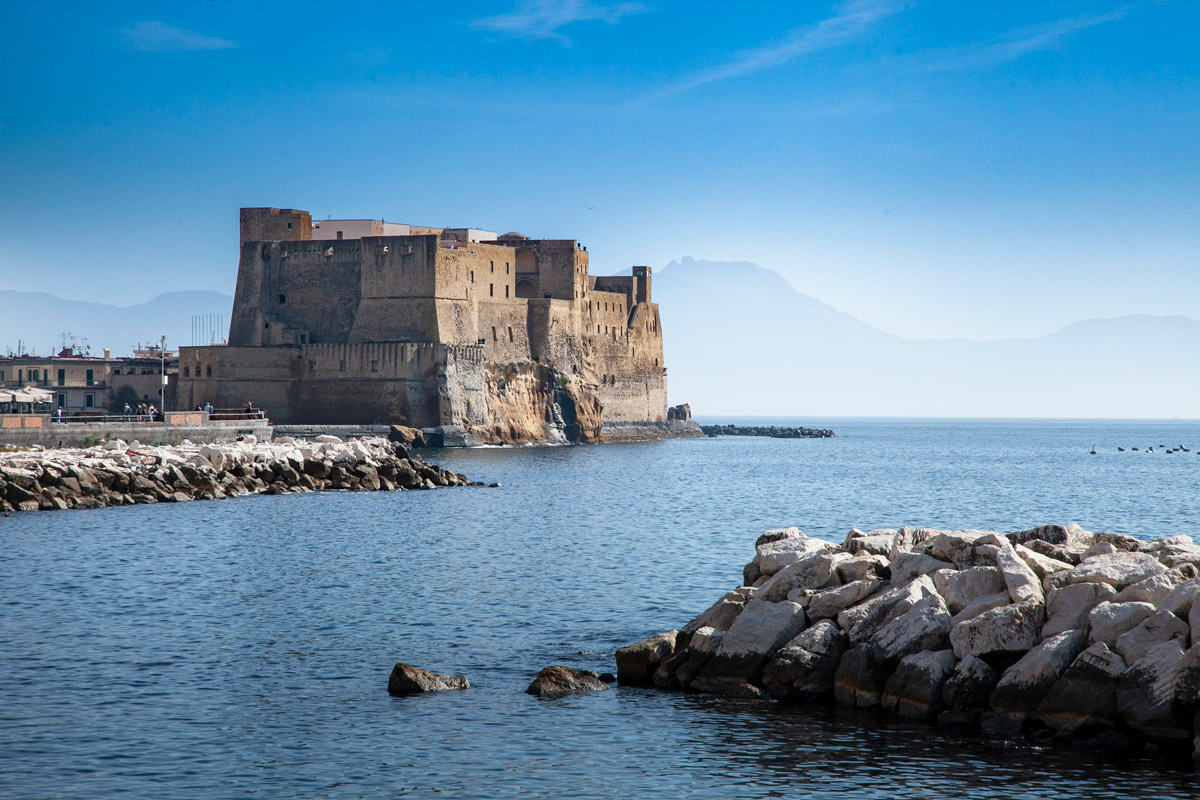
\includegraphics[width=\textwidth]{images/input_image_t5.jpg}
        \caption{(a) Input image.}
        \label{fig:test_5_input}
    \end{minipage}
    \hfill
    \begin{minipage}[b]{0.45\textwidth}
        \centering
        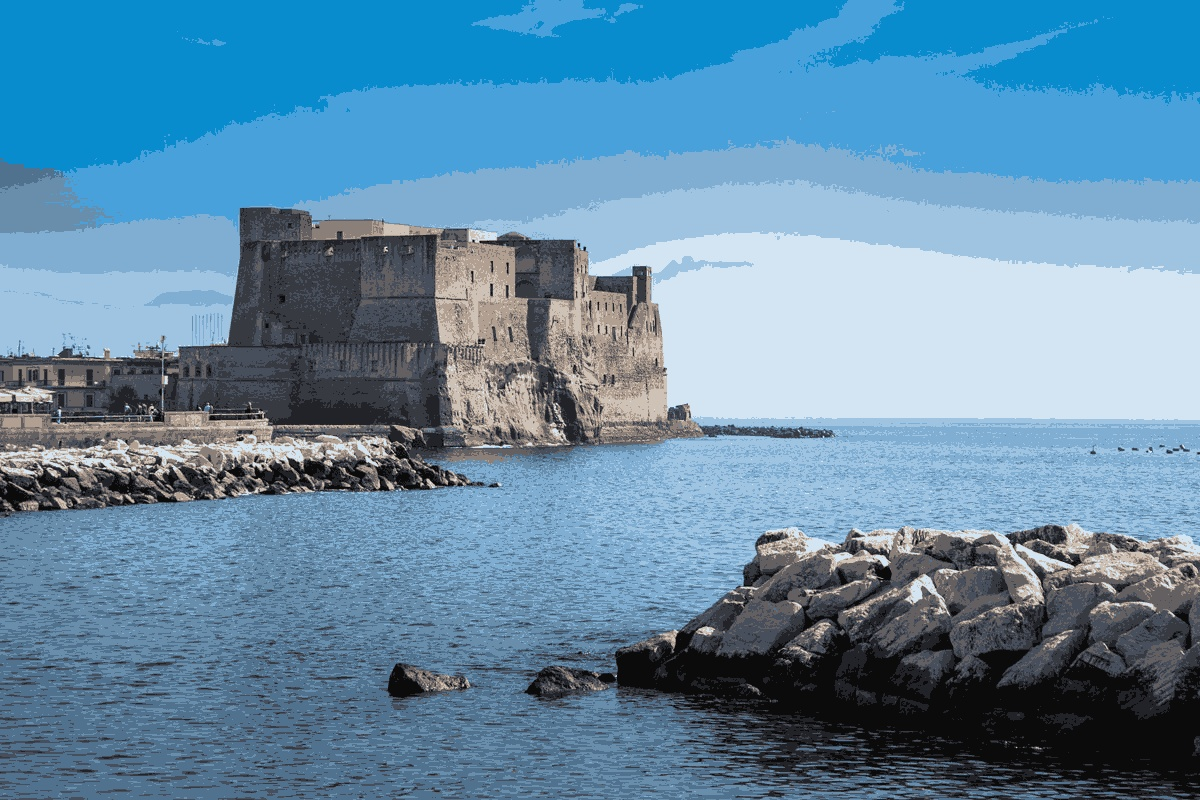
\includegraphics[width=\textwidth]{images/output_image_t5.jpg}
        \caption{(b) Output image.}
        \label{fig:test_5_output}
    \end{minipage}
    \end{figure}


    \begin{table}[H]
        \centering
        \begin{tabular}{|l|l|}
        \hline
        \textbf{Input Info}                    & \textbf{Value}                       \\ \hline
        Session ID                             & 4                                     \\ \hline
        Image width                            & 1200px                                \\ \hline
        Image height                           & 800px                                 \\ \hline
        Image channels                         & RGB (3 channels)                      \\ \hline
        \#Clusters                             & 15                                    \\ \hline
        \#Iterations                           & 100                                   \\ \hline
        \#Threads                              & 128                                   \\ \hline
        Random seed                            & 200                                   \\ \hline
        \end{tabular}
        \caption{Session information}
        \label{tab:session_information_test5}
        \end{table}
        

        \subsection{GeForce 1660}

        \begin{table}[H]
            \centering
            \begin{tabular}{|l|l|}
            \hline
            \textbf{Metric}                         & \textbf{Value}                       \\ \hline
            Execution time (Parallel version)       & ~974ms (0.9s)                        \\ \hline
            Execution time (Sequential version)     & ~4860ms (4.86s)                      \\ \hline
            Delta time                               & +3886ms (+3.88s)                     \\ \hline
            Speedup                                  & 4.9                                   \\ \hline
            \end{tabular}
            \caption{Performance Metrics on \textbf{Machine 1}}
            \label{table:performance_metrics_test5_machine1}
        \end{table}
        
        
        \subsection{Geforce 4060}
        
        \begin{table}[H]
            \centering
            \begin{tabular}{|l|l|}
            \hline
            \textbf{Metric}                         & \textbf{Value}                       \\ \hline
            Execution time (Parallel version)       & ~933ms (0.9s)                        \\ \hline
            Execution time (Sequential version)     & ~17940ms (17.9s)                     \\ \hline
            Delta time                               & +17000ms (+17s)                      \\ \hline
            Speedup                                  & 19.2                                  \\ \hline
            \end{tabular}
            \caption{Performance Metrics on \textbf{Machine 2}}
            \label{table:performance_metrics_test5_machine2}
        \end{table}
        
        
        \subsection{Quadro K5000}
        
        \begin{table}[H]
            \centering
            \begin{tabular}{|l|l|}
            \hline
            \textbf{Metric}                         & \textbf{Value}                       \\ \hline
            Execution time (Parallel version)       & ~2806ms (2.80s)                      \\ \hline
            Execution time (Sequential version)     & ~44190ms (44.19s)                    \\ \hline
            Delta time                               & +41384ms (+41.38s)                   \\ \hline
            Speedup                                  & 15.74                                 \\ \hline
            \end{tabular}
            \caption{Performance Metrics on \textbf{Machine 3}}
            \label{table:performance_metrics_test5_machine3}
        \end{table}
\subsection{Conclusion}        
In Test 5, the results demonstrate significant improvements in execution times across all machines when using parallel processing. The GeForce 1660 achieved a speedup of 4.9, showing a solid performance improvement, while the Geforce 4060 outperformed the other GPUs with a remarkable speedup of 19.2. The Quadro K5000 also demonstrated a strong performance with a speedup of 15.74, illustrating the effectiveness of parallel computation for reducing processing times.

The varying speedups suggest that the Geforce 4060 is the most efficient for this task, highlighting the benefits of modern GPUs with more computational power. The results further emphasize the importance of parallel processing in accelerating image processing tasks, particularly when working with larger datasets or more iterations. This test reinforces the continued need for optimization, as well as the value of selecting the appropriate hardware to maximize computational efficiency.

\section{Test 6}
\begin{figure}[H]
    \centering
    \begin{minipage}[b]{0.45\textwidth}
        \centering
        
\includegraphics[width=\textwidth]{images/input_image_t6.jpg}
        \caption{(a) Input image.}
        \label{fig:test_6_input}
    \end{minipage}
    \hfill
    \begin{minipage}[b]{0.45\textwidth}
        \centering
        \includegraphics[width=\textwidth]{images/output_image_t6.jpg}
        \caption{(b) Output image.}
        \label{fig:test_6_output}
    \end{minipage}
    \end{figure}

    \begin{table}[H]
        \centering
        \begin{tabular}{|l|l|}
        \hline
        \textbf{Input Info}                    & \textbf{Value}                       \\ \hline
        Session ID                             & 5                                     \\ \hline
        Image width                            & 7680px                                \\ \hline
        Image height                           & 4320px                                \\ \hline
        Image channels                         & RGB (3 channels)                      \\ \hline
        \#Clusters                             & 15                                    \\ \hline
        \#Iterations                           & 100                                   \\ \hline
        \#Threads                              & 128                                   \\ \hline
        Random seed                            & 200                                   \\ \hline
        \end{tabular}
        \caption{Session information}
        \label{tab:session_information_test6}
        \end{table}
        

        \subsection{GeForce 1660}

        \begin{table}[H]
            \centering
            \begin{tabular}{|l|l|}
            \hline
            \textbf{Metric}                         & \textbf{Value}                       \\ \hline
            Execution time (Parallel version)       & ~39678ms (38.93s)                    \\ \hline
            Execution time (Sequential version)     & ~163920ms (2.73 minutes)             \\ \hline
            Delta time                               & +124242ms (+2.07 minutes)           \\ \hline
            Speedup                                  & 4.13                                  \\ \hline
            \end{tabular}
            \caption{Performance Metrics on \textbf{Machine 1}}
            \label{table:performance_metrics_test6_machine1}
        \end{table}
        
        
        \subsection{Geforce 4060}
        
        \begin{table}[H]
            \centering
            \begin{tabular}{|l|l|}
            \hline
            \textbf{Metric}                         & \textbf{Value}                       \\ \hline
            Execution time (Parallel version)       & ~39678ms (39.6s)                     \\ \hline
            Execution time (Sequential version)     & ~630806ms (10.5 minutes)             \\ \hline
            Delta time                               & +591128ms (+9.8 minutes)             \\ \hline
            Speedup                                  & 15.89                                 \\ \hline
            \end{tabular}
            \caption{Performance Metrics on \textbf{Machine 2}}
            \label{table:performance_metrics_test6_machine2}
        \end{table}
        
        
        \subsection{Quadro K5000}
        
        \begin{table}[H]
            \centering
            \begin{tabular}{|l|l|}
            \hline
            \textbf{Metric}                         & \textbf{Value}                       \\ \hline
            Execution time (Parallel version)       & ~100197ms (1.66 minutes)             \\ \hline
            Execution time (Sequential version)     & ~1481520ms (24.69 minutes)           \\ \hline
            Delta time                               & +1381323ms (+23.02 minutes)          \\ \hline
            Speedup                                  & 14.78                                 \\ \hline
            \end{tabular}
            \caption{Performance Metrics on \textbf{Machine 3}}
            \label{table:performance_metrics_test6_machine3}
        \end{table} 
\subsection{Conclusion}
Test 6 highlights the substantial performance improvements achieved through parallel processing. The GeForce 1660 demonstrated a speedup of 4.13, reflecting moderate acceleration, while the Geforce 4060 and Quadro K5000 showed much stronger improvements, with speedups of 15.89 and 14.78, respectively. This indicates that the more powerful GPUs, particularly the Geforce 4060, offer the most significant performance gains, reducing execution times dramatically.
The results reinforce the value of parallelization for processing large image datasets, as demonstrated by the substantial reductions in execution time when using parallel versions over sequential ones. This test further emphasizes the importance of selecting high-performance GPUs to achieve optimal efficiency for complex image processing tasks, particularly with larger images or higher iterations.        

\newpage
\section{GPUs comparison}
In this section, we present a comparison of the performance across different GPU models (GeForce 1660, GeForce 4060, and Quadro K5000) based on the execution times and overall efficiency during the various test sessions.

Figure \ref{figure:execution_time_per_session} shows the execution times for each machine across the different test sessions. From the graph, it is evident that the GeForce 4060 consistently performs faster than both the GeForce 1660 and the Quadro K5000, with the largest differences observed in the more demanding sessions (those with larger image sizes or higher iteration counts). The GeForce 1660, while generally slower, still delivers improved performance compared to the sequential version.

\begin{figure}[H]
    \centering
    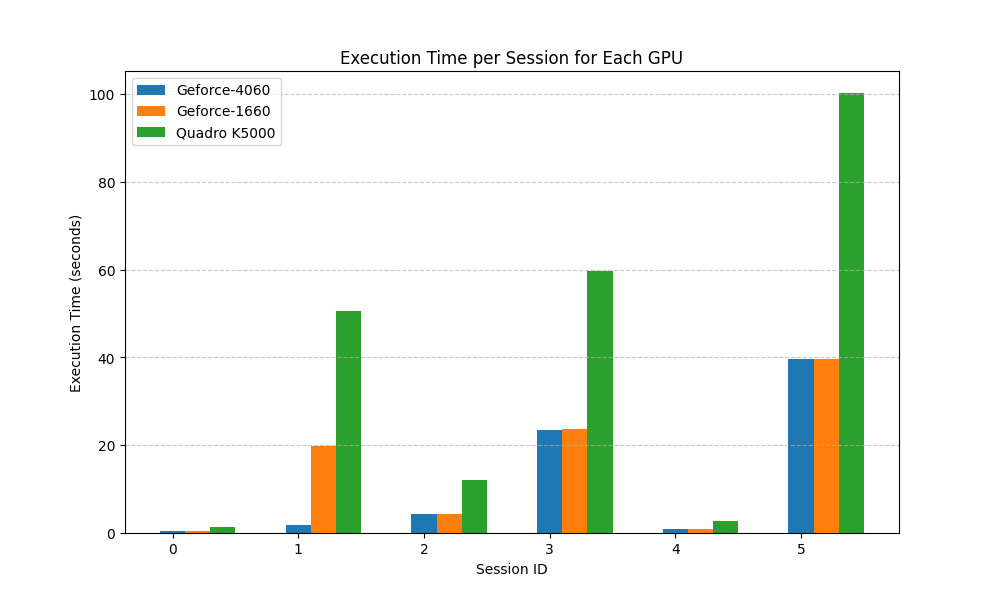
\includegraphics[width=0.8\textwidth]{images/execution_time_per_session.jpeg}
    \caption{Execution time of different machines per session}
    \label{figure:execution_time_per_session}
\end{figure}

Figure \ref{figure:execution_time_distribution} illustrates the distribution of the total execution time for each machine. This chart provides further insights into the variance in performance across the different sessions. We can observe that while the GeForce 4060 maintains a more consistent and lower execution time, the Quadro K5000 shows a larger variation in its performance across the sessions, indicating that its speedup might be more dependent on the specific task or workload.
\begin{figure}[H]
    \centering
    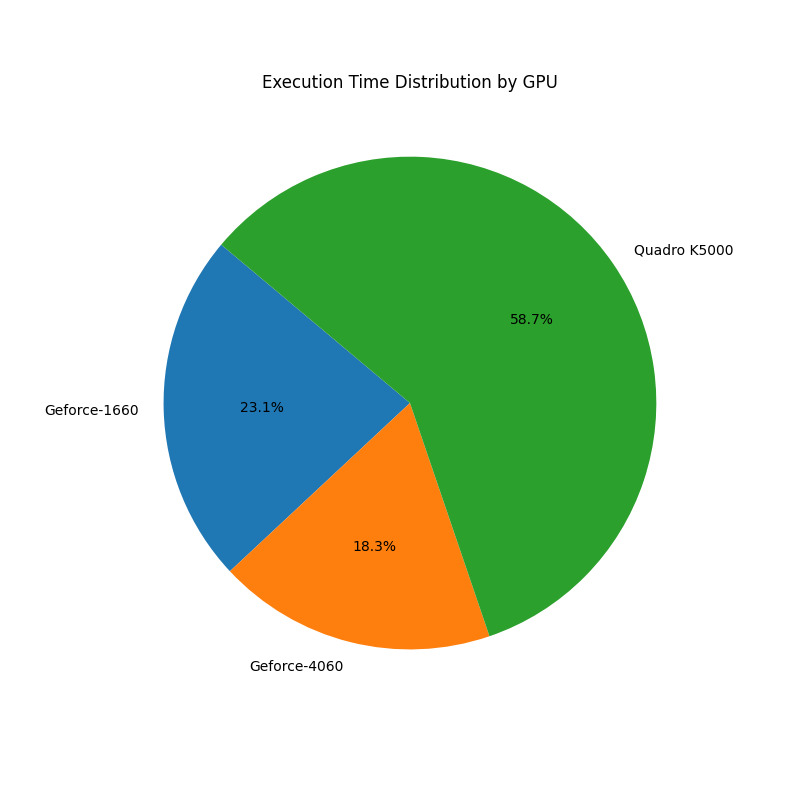
\includegraphics[width=0.6\textwidth]{images/execution_time_distribution.jpeg}
    \caption{Total execution time distribution}
    \label{figure:execution_time_distribution}
\end{figure}

Figure \ref{figure:average_gpu_time} compares the average GPU time spent processing tasks across all sessions for each GPU. As expected, the GeForce 4060 exhibits the lowest average GPU time, followed by the GeForce 1660 and Quadro K5000. This result highlights the efficiency of the newer, more powerful GeForce 4060 in handling image processing tasks and emphasizes the role of GPU architecture in optimizing computational workloads.
\begin{figure}[H]
    \centering
    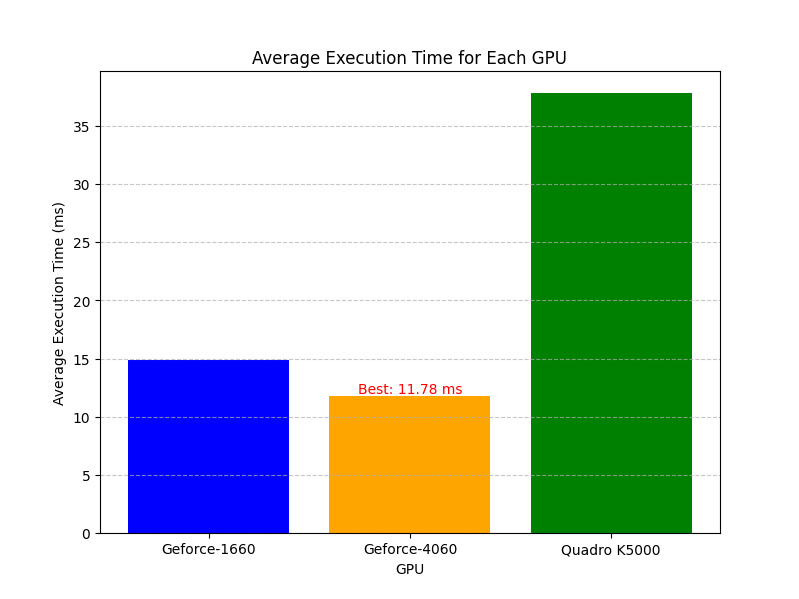
\includegraphics[width=0.6\textwidth]{images/average_gpu_time.jpeg}
    \caption{Average GPU time comparison}
    \label{figure:average_gpu_time}
\end{figure}

\section{Discussion}
We evaluated the performance of various GPU models (GeForce 1660, GeForce 4060, and Quadro K5000) across several test scenarios, analyzing the effectiveness of parallel processing for image-based tasks. The results clearly demonstrate the significant advantages of using parallel processing over sequential approaches, with notable speedup improvements observed across all GPU models.
Key findings include:
\begin{itemize}
    \item The GeForce 4060 consistently outperformed the other GPUs, delivering the highest speedup and reducing execution times substantially, especially with larger image sizes and higher iteration counts.
    \item The Quadro K5000, while slower than the GeForce 4060, still demonstrated a solid performance improvement over the sequential version, making it a strong option for large-scale image processing tasks.
    \item The GeForce 1660, although providing modest speedups, was still able to achieve faster execution times than the sequential version, highlighting the benefit of parallelization even with mid-range GPUs.
\end{itemize}

These results underscore the importance of parallel computing for image processing tasks, where GPU acceleration plays a pivotal role in reducing computation time and enabling real-time or near-real-time processing. The choice of GPU significantly impacts performance, with high-end models like the GeForce 4060 providing the most noticeable improvements.
